\chapter{Ondes mécaniques}

\newpage

\section{Longueur d'un son}

Une feuille métallique rectangulaire, de masse surfacique $\sigma=7,8\times10{-2}$kg.m$^{-3}$, de dimensions $l\times L=2\times2$m suivant les axes $x$ et $y$, est fixée sur un support le long des deux côtés de dimension $L=2$m. La feuille est tendue entre ces deux supports jusqu'à une tension $T_0=3,0\times10^6$N le long de l'axe $x$.

\begin{figure}[h]
\centering
  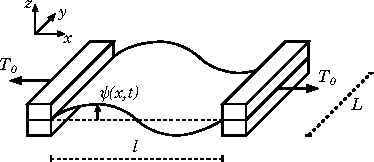
\includegraphics[scale=1.9]{onde_meca_feuille_vibrante.pdf}
\end{figure}

Lorsqu'on frappe sur cette plaque, on suppose qu'elle ne peut vibrer que suivant la direction $x$. Le son émis se propage à la vitesse $c_0=343$m.s$^{-1}$ dans l'air environnant dont la masse volumique est $\rho_0=1,3$kg.m$^{-3}$.

On frappe la plaque de sorte à ce que le son atteigne un volume sonore de 70dB à 1m de distance, durant les premiers instants. Estimer le temps au bout duquel le son ne sera plus perceptible.

\newpage

\begin{correction}

L'idée est de considérer la vibration mécanique de la feuille s'amortitissant en cédant de la puissance sonore à l'air, que l'on peut quantifier à partir du vecteur de Poynting sonore $\vec{Pi}$.

On commence par évaluer la fréquence de l'onde : $f\simeq c/\lambda$, où $\lambda\simeq 2l$ est la longueur d'onde du fondamental et $c$ la vitesse de l'onde mécanique dans la plaque, donnée par $c=\sqrt{T_0/\mu}=\sqrt{T_0/\sigma L}\simeq4,3\times10^3$m.s$^{-1}$. La plaque vibre donc à la fréquence $f\simeq 1,1$kHz, donc la longueur d'onde de l'onde sonore est $\lambda_0=c/f_0\simeq31$cm. On peut considérer que $\lambda_0 \ll L$, l'onde sonore est émise par un plan, donc est une onde "localement" plane. 

Avec la géométrie du problème, le champ de vitesse de cette onde peut s'écrire :
\begin{align*}
	\vec{v}(x,z,t)=\frac{d\psi}{dt}\left(x,t-\frac{z}{c}\right) \vec{e}_z
\end{align*}
car sur la surface de la feuille (le plan $z=0$), par conservation du débit, $\vec{v}(x,z=0,t)=\frac{d\psi}{dt}(x,t)$ où $\psi$ représente la hauteur de la vibration de la feuille par rapport à l'équilibre. Le champ de vitesse à une distance $z$ de la feuille est donc ensuite simplement décalé de $t-\frac{z}{c}$. 

La puissance propagée par l'onde sonore est donnée par le vecteur de Poynting $\vec{\Pi(x)}=p\vec{v}$. En $z=\psi$, cette puissance est :
\begin{align*}
	\vec{\Pi(x)}&=p(x,\psi,t)\vec{v}(x,\psi,t) \\
	&=Z_0v^2(x,\psi,t)\vec{e}_z \\
	&=Z_0\left( \frac{d\psi}{dt}\right)^2\vec{e}_z
\end{align*}
La puissance transmise à l'onde sonore est perdue par la plaque. Pour un élément de surface $dS=dx\times L$ de la feuille, la puissance cédée à l'onde sonore est :
\begin{align*}
	dP&=-||\vec{\Pi(x)}||dxL \\
	&=-Z_0dxL\left( \frac{d\psi}{dt}\right)^2 \\
	&=df_{frott.}\frac{d\psi}{dt}
\end{align*}
On peut écrire $dP$ comme la puissance cédée par l'élément de feuille $dx\times L$ se déplaçant à la vitesse $\frac{d\psi}{dt}$ par une force de frottement $df_{frott.}=-Z_0dxL\frac{d\psi}{dt}(x,t)$ :

On part maintenant sur l'analyse de la feuille. Pour un élément de feuille $dx\times L$, on peut appliquer le même raisonnement que pour le cas de la corde vibrante. Le PFD donne alors :
\begin{align*}
	\sigma dx  L\frac{d^2\psi}{dt^2}=-T(x)\sin\alpha(x)+T(x+dx)\sin\alpha(x+dx)-Z_0dxL\frac{d\psi}{dt}(x,t)
\end{align*}
On trouve alors, avec le raisonnement habituel de la corde vibrante :
\begin{align*}
	\frac{d^2\psi}{dt^2}=\frac{T_0}{\sigma L}\frac{d^2\psi}{dx^2} -\frac{Z_0}{\sigma}\frac{d\psi}{dt}(x,t)
\end{align*}
On notera $c^2=T_0/\sigma L$. On cherche alors des solutions stationnaires sous la forme $\psi(x,t)=f(x)g(t)$. En injectant dans l'équation précédente, et en divisant par $\psi(x,t)$, on obtient :
\begin{align*}
	\frac{g"(t)}{g(t)}+\frac{Z_0}{\sigma}\frac{g'(t)}{g(t)}=c^2\frac{f"(x)}{f(x)}
\end{align*}
La partie gauche de l'équation étant indépendante de $x$, on peut résoudre l'équation différentielle sur $f$. Avec les conditions aux limites, on trouve $f(x)=A\sin\left(\frac{n\pi x}{l}\right)$, avec $n\in\mathbb{Z}$. L'équation sur la fonction $g$ devient :
\begin{align*}
	g"(t)+\frac{Z_0}{\sigma}g'(t)+\frac{\pi^2n^2c^2}{l^2}=0
\end{align*}
La solution générale de cette équation est :
\begin{align*}
	g(t)=B\cos(\omega t +\phi)e^{-t/\tau}
\end{align*}
où $\tau=\frac{\sigma}{2Z_0}$.

\end{correction}